\begin{figure}[h!]
\textbf{Tema d'Esame di Gennaio 2015}\\ \\
Del propanolo, densità $d=803 g/cm^3$ scorre attraverso un tubo orizzontale che si restringe come in figura e ha una variazione di quota di $50cm$. La sezione $A1=1.60\cdot 10^3m^2$ e $A2=\frac{A1}{2}$. La differenza di pressione nel tubo tra il punto a sezione larga e il punto a sezione stretta è $8240Pa$. Qual'è la portata del propanolo del tubo?
\\
	\begin{center}
		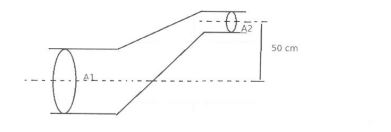
\includegraphics[scale=1.1]{ES4/GEN042015.jpg}
	\end{center}
\end{figure}

\begin{figure}[h!]
\textbf{Tema d'Esame di Febbraio 2015}\\ \\
 Un rubinetto di sezione $S = 1 cm^2$
 è inserito nel fondo di una (grande) cisterna aperta
superiormente. Il livello dell'acqua nella cisterna è $H = 4 m$. Il getto d'acqua uscente dal
rubinetto è diretto verticalmente verso il basso. Trascurando tutti I possibili attriti, si
determini la sezione $Sh$ del getto d'acqua dopo che questo è sceso verso il basso di un tratto
$h = 20 cm$. (Poiché la cisterna è grande, si può assumere che il livello dell'acqua $H$ resti
costante).
\\
\end{figure}

\begin{figure}[h!]
\textbf{Tema d'Esame di Giugno 2015}\\ \\
Un corpo sferico di massa $400kg$ è immerso in acqua ($\rho_{H2O}=1000kg/m^3$)e il raggio del corpo è $r=0.1m$. Il corpo viene appeso ad un palloncino piano d'aria ($\rho_{aria}=1.2kg/m^3$). Calcolare il raggio minimo del palloncino per cui i due corpi non vadano a fondo (il palloncino è sferico e non ha massa).
\\
\begin{center}
		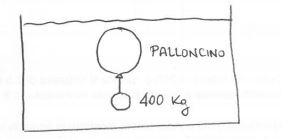
\includegraphics[scale=1.3]{ES4/GIU042015.jpg}
	\end{center}
\end{figure}

\begin{figure}[h!]
\textbf{Tema d'Esame di Luglio 2015}\\ \\
In un tubo orizzontale che presenta sezioni $S_1=10cm^3$ e $S_2=5cm^3$ scorre dell'acqua (densità $1g/cm^3$) con una portata $Q=0.82kg/s$. Determinare la differenza di pressione esistente tra le due sezioni.
\\
\begin{center}
		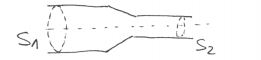
\includegraphics[scale=1.6]{ES4/LUG042015.jpg}
	\end{center}
    
    \begin{boxed}
\textbf{Soluzione:}\\
Conversioni\\
$\rho_{acqua}=1g/cm^3=\frac{1\cdot 10^{-3}}{1\cdot 10^{-6}}kg/m^3=1\cdot 10^3kg/m^3 $\\\\
$Q=0.82kg/s= \frac{Q}{\rho}=\frac{0.82kg/s}{1\cdot10^3kg/m^3}=8.2\cdot10^{-4}m^3/s$\\ \\
$S_1=10cm^2 =1\cdot 10^{-3}m^2$\\
$S_2=5cm^2 =5\cdot 10^{-4}m^2$\\

Sapendo che vale:\\
$A_1\cdot V_1=A_2\cdot V_2$\\
$p_1 + \frac{1}{2}\cdot \rho \cdot v^2_1 = p_2 + \frac{1}{2}\cdot \rho \cdot v^2_2 \qquad \Delta p=\frac{1}{2}\cdot \rho \cdot (v^2_2 - v^2_1)$\\
Essendo entrambe le velocità incognite le ricaviamo da:\\
$v_1=\frac{Q}{A_1}=\frac{8.2\cdot10^{-4}m^3/s}{1\cdot 10^{-3}m^2}=0.82m/s$\\
$v_2=\frac{Q}{A_2}=\frac{8.2\cdot10^{-4}m^3/s}{5\cdot 10^{-4}m^2}=1.64m/s$\\
Tornando alla formula di prima otteniamo che:\\
$\Delta p=\frac{1}{2}\cdot 10^3kg/m^3 \cdot ((1.64m/s)^2 - (0.82m/s)^2)=\frac{1}{2}\cdot 10^3kg/m^3 \cdot (2.01m^2/s^2) =1.008Pa$
\end{boxed}
\end{figure}